

\section{Methods}

% We should probably cite \citet{braun2006using} here...
We aim to understand perceptions of computer science students about climate change and how their field affects and is affected by it. To gauge these opinions, we conducted semi-structured interviews with students varying from undergraduate and graduate levels. In this section we describe how we collected the data, extracted themes and deduced results from the data.

\subsection{Materials and Procedure}
The semi-structured interview included \oldstylenums{13} questions that are tailored to provide insights for our research questions. Q1-Q5 collected demographic information on participants (name, gender, age and area of expertise). Q6 was a general warm-up question about the participant’s professional plan for the future. Q7-Q9 were used to answer “How climate change was perceived in daily life?”. Q10-Q11 aimed to find out “How climate change would influence their area of expertise?” Q12-Q13 discovered “What opportunities were presented in terms of alleviating the effects of climate change?”

There were a total of \oldstylenums{5} interviews conducted. They were semi-structured and conducted online using a video messaging platform called Zoom, all lasting around \oldstylenums{20} minutes each. The interviews were recorded with permission and transcribed afterwards. 

% \footnote{https://zoom.us/}

\subsection{Analysis}
After conducting and transcribing the interviews, we analyzed them using a bottom-up, inductive process, as per \citet{braun2006using}.

\subsubsection{Generating and collating initial codes} Interviews were bundled into one document. Each author was given a copy of this final transcript and annotated them individually without communication or interference from other authors, extracting initial codes from the interviews. After being generated, they were collated and collapsed by the similarity of their content, then displayed as sticky notes using a collaborative whiteboard platform.
% called Miro \footnote{https://www.miro.com}. %Figure \ref{fig:initial-codes} shows an example of initial codes created by one of the authors.

% \begin{figure}
%     \centering
%     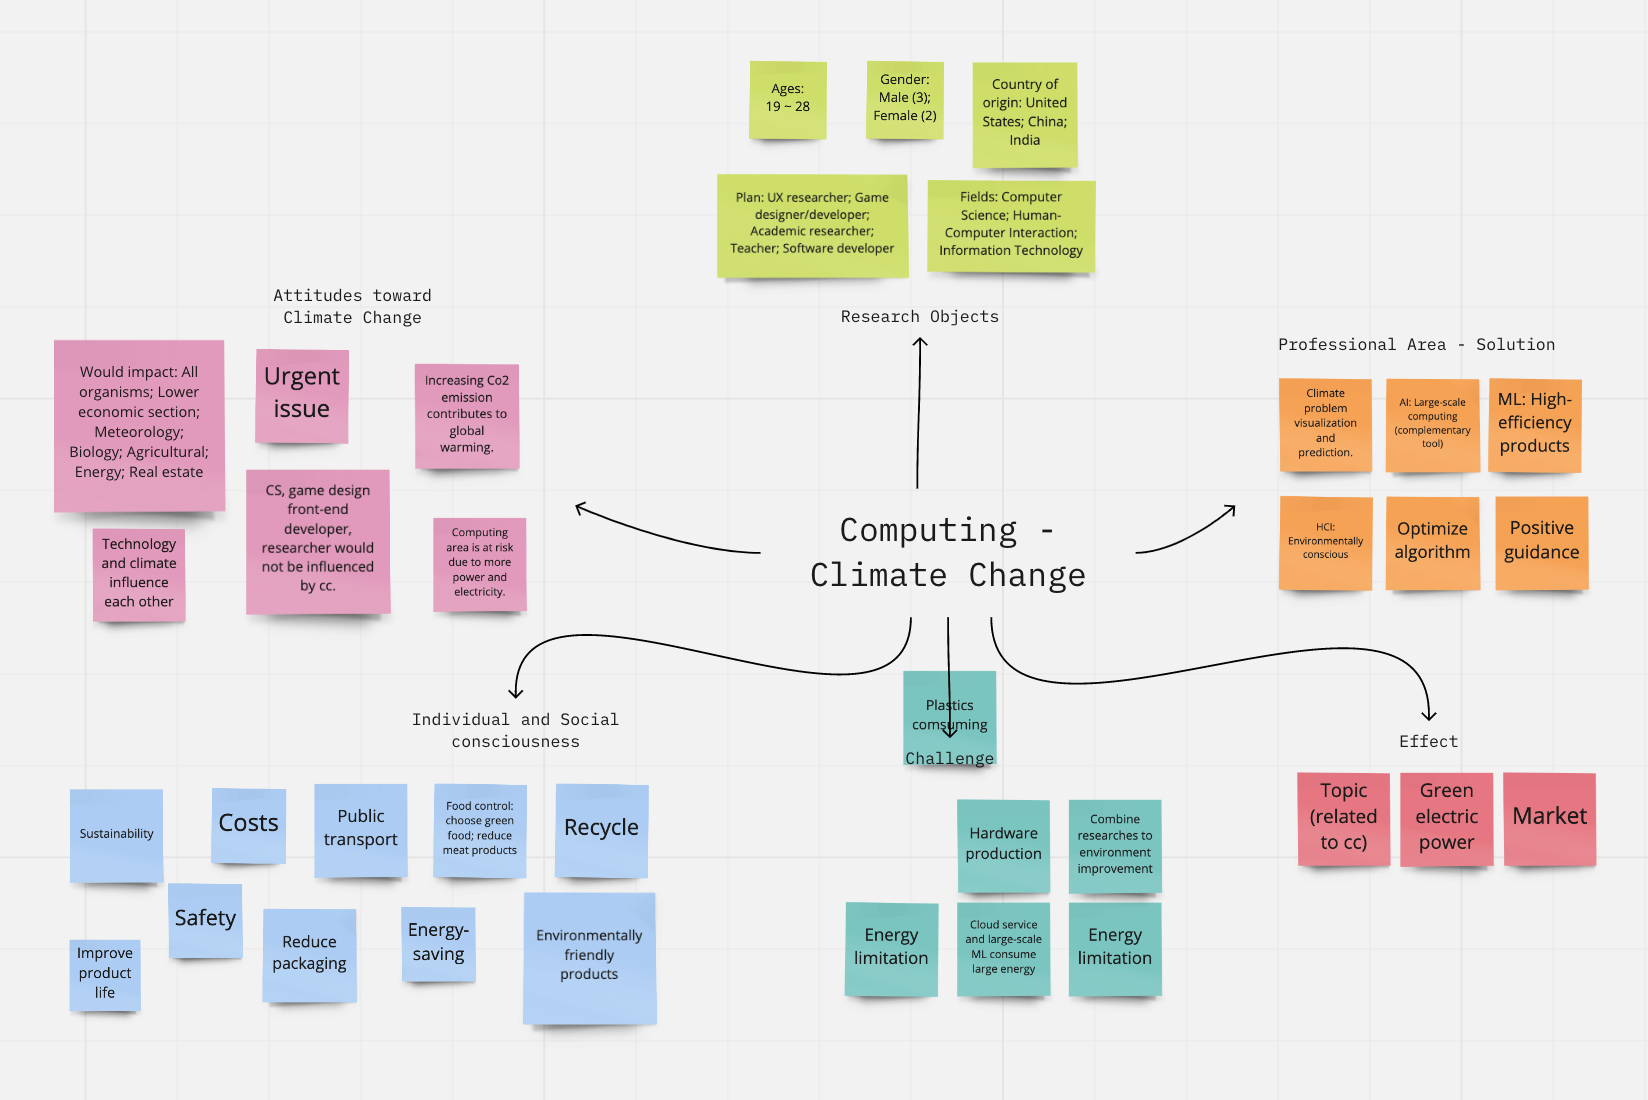
\includegraphics[scale = 0.2]{Figures/Initial Codes.png}
%     \caption{Example of Initial Codes}
%     \label{fig:initial-codes}
% \end{figure}

\subsubsection{Defining themes}

After pasting all codes in the same place, we created an overall coding diagram to identify similarities that allowed thematic grouping. We ended up identifying four major categories, to which we attached the codes' post-its. %Figure \ref{fig:theme-codes} illustrates this process. 
All four categories provide insights to our research questions for the ``perception of climate change'' and the ``impact on area of expertise.'' Finally, in writing the report, we established the final two themes, \emph{Unsystematic risks} and \emph{Limits to action}, with which we wrote our final analysis.

% \begin{figure}
%     \centering
%     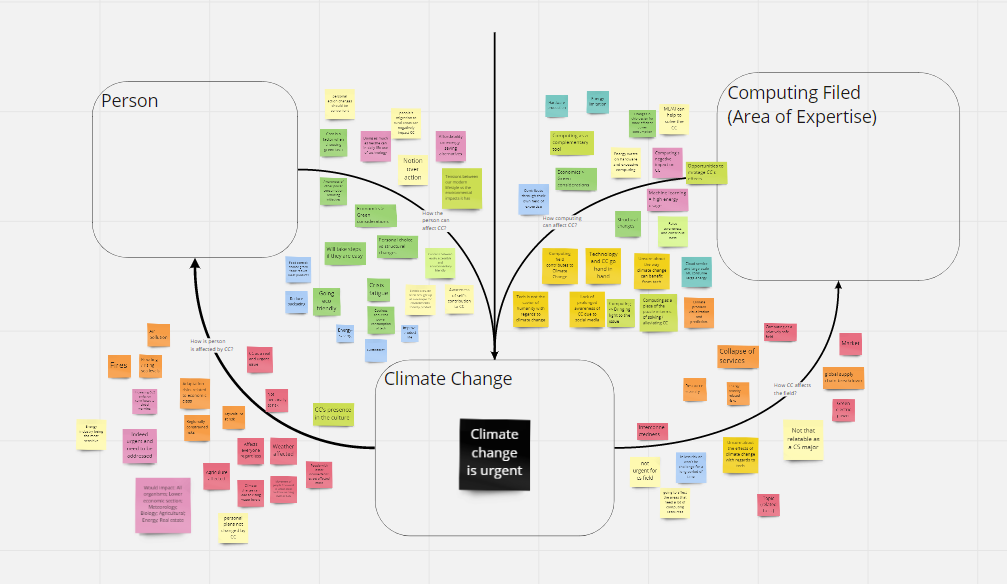
\includegraphics[scale = 0.2]{Figures/codes.png}
%     \caption{Themes and their corresponding codes}
%     \label{fig:theme-codes}
% \end{figure}


